% commento

\section{Sezione d'urto}

\paragraph{Elemento X} ha un numero di massa $A$ che corrisponde alla somma di \emph{neutroni} e \emph{protoni} nel nucleo ed un numero atomico $Z$ che è il numero di \emph{protoni} nel nucleo, per cui si scrive:
$$^{A}_{Z} X$$
in un atomo neutro il numero atomico corrisponde anche al numero di \emph{elettroni}.


\subsection{Esperimento di Rutherford}
Quando Rutherford iniziò i suoi studi l'idea di nucleo era quella di una sfera di carica positiva con all'interno degli elettroni negativi (modello a panettone).
Si sapeva sapeva inoltre che i nuclei emettono particelle ed erano conosciute le emissioni $\alpha,\gamma ,\beta$.
L'intuizione di Rutherford fu di utilizzare il decadimento dei nuclei $\alpha$ ed adottando un approccio statistico per ovviare al problema di non conoscere la posizione esatta delle particelle.

Nell'esperimento, Rutherford, utilizza un nucleo di \textbf{Radio} (Ra) con numero di massa $A=226$ e numero atomico $Z=88$, ovvero $^{226}_{88} Ra$ .
Il \emph{decadimento} che avviene è il seguente
\begin{equation}
^{226}_{88} Ra \longrightarrow ^{222}_{86}Rn + ^{4}_{2}He + Q
\end{equation}
nella reazione si conserva il numero di massa totale $ 226 = 222 + 4 $ e si conserva la carica totale $ 88 = 86 + 2 $;
$Q$ è il calore emesso dalla reazione esotermica/spontanea, equivalente all'energia data dalla differenza di massa iniziale e finale. 
L'energia cinetica rilasciata nel decadimento che viene trasferita alla particella $\alpha$ è pari a $T = \SI{4.76}{MeV}$.
Un fascio collimato di particelle $\alpha$ viene indirizzato contro un \emph{target} (lastra sottile di oro).
Il fascio uscente veniva rivelato da uno schermo di ZnS, mobile su tutto l'angolo solido.
Il fatto sorprendente e inaspettato era che una piccolissima porzione di particelle veniva deflessa ad angoli impossibili per il modello a panettone (si rilevano particelle pure a 180° ovvero fenomeni di back scattering), in quanto l'energia di repulsione non sarebbe stata sufficiente.
Essenziale fu l'intuizione di Rutherford che non prese tale dato come errore ma capì che si trattava di particelle reali.
\begin{figure}[hbtp]
\centering
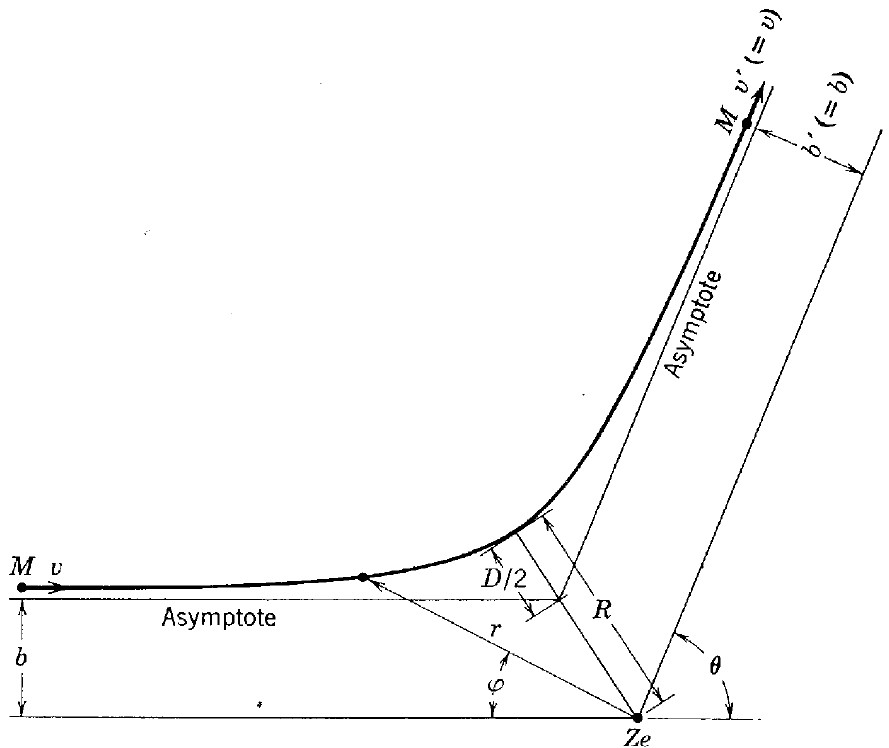
\includegraphics[width=200pt]{fig1_01}
\caption{Traiettoria iperbolica della particella in interazione con un nucleo}
\label{fig:1.1}
\end{figure}
La sezione d'urto di Rutherford fu calcolata inizialmente sfruttando semplicemente la meccanica classica.
In figura viene mostrato lo scattering di una particella $\alpha$ di massa M e carica +ze, passante vicino ad un nucleo di carica +Ze.
Il nucleo è fissato al centro del sistema di coordinate.
Prima e dopo la collisione la particella avrà una traiettoria rettilinea (prima con velocità v poi con velocità v') in quanto la forza coulombiana è trascurabile dopo una certa distanza .
Per determinare la posizione della particella si sfruttano le coordinate polari $r(t), \varphi$. 
La distanza tra la traiettoria della particella e la linea parallela passante per il nucleo (asse orizzontale del sistema) è definita come il \emph{parametro d'impatto} $b$.
L'angolo di scattering $\theta$ è dato dall'intersezione dell'asse orizzontale con la parallela alla traiettoria finale passante per il nucleo.

Siccome il nucleo viene considerato fisso, l'energia cinetica finale della particella deve essere identica a quella iniziale. 
Velocità e parametro d'impatto sono costanti prima e dopo l'impatto a causa della conservazione dell'energia cinetica e del momento angolare.
\[Mvb=Mv'b'=L \hspace{1cm} \frac{1}{2}Mv^2=\frac{1}{2}Mv'^2\]
(si ha la conservazione del momento angolare perché in presenza di una forza centrale; $dL/dt=\bar r \times \bar F (r)=0$; raggio e forza sono sempre paralleli).

Sfruttando nuovamente il momento angolare si cerca ora di ottenere il differenziale del tempo
\[|L|=|\bar r \times m\bar v|=mvb=mv_\perp r=m\omega r^2=m\frac{d\varphi}{dt}r^2\]
dove $v_\perp=\omega r$ e $\omega=d\varphi/dt$. 
Si ottinene quindi
\[\frac{d\varphi}{dt}=\frac{vb}{r^2}\hspace{0.2cm}\to\hspace{0.2cm} dt=d\varphi \frac{r^2}{vb}\]
Si passa ora ad introdurre l'interazione elettromagnetica. 
Verrà qui sfruttato il teorema dell'impulso
\[\Delta p=\int F_n dt\hspace{1cm}F_n=F\cos\varphi\]
dove F è la forza coulombiana
\[F=\frac{1}{4\pi\varepsilon_0}\frac{zZe^2}{r^2}\]
\[\Delta p=\int_{-\infty}^{+\infty} \frac{1}{4\pi\varepsilon_0}\frac{zZe^2}{r^2}\cos\varphi dt\]
Possiamo quindi sostituire la formula per $dt$ trovata sopra all'interno dell'integrale appena ricavato prestando ovviamente attenzione agli estremi d'integrazione 
\[t\to -\infty\hspace{2cm}\varphi\to-\frac{1}{2}(\pi-\theta)\]
\[t\to +\infty\hspace{2cm}\varphi\to+\frac{1}{2}(\pi-\theta)\]
\[\Delta p=\int _{-\frac{1}{2}(\pi-\theta)}^{+\frac{1}{2}(\pi-\theta)}\frac{1}{4\pi\varepsilon_0}\frac{zZe^2}{vb}\cos\varphi d\varphi\]
Rinominando tutte le costanti dell'integrale come A si ottiene
\[\Delta p=A[\sin\varphi] _{-\frac{1}{2}(\pi-\theta)}^{+\frac{1}{2}(\pi-\theta)}=A\biggl[\sin\left(\frac{\pi}{2}-\frac{\theta}{2}\right)-\sin\left(\frac{\pi}{2}+\frac{\theta}{2}\right)\biggl]=2A\cos\frac{\theta}{2}\]
A questo punto è necessario ricavare la variazione della quantità di moto proiettando la quantità di moto sulla normale
\[p_f-p_i=2mv\sin\frac{\theta}{2}\]
abbiamo ottenuto così che
\[2mv\sin\frac{\theta}{2}=2A\cos\frac{\theta}{2}\to 2mv\sin\frac{\theta}{2}=\frac{zZe^2}{4\pi \varepsilon_0vb}\cos\frac{\theta}{2}\]
\[\tan\frac{\theta}{2}=\frac{zZe^2}{4\pi\varepsilon_0mv^2}\frac{1}{b}\to\tan\frac{\theta}{2}=K\frac{1}{b}\]
Da quest'ultima formula si può vedere che se $b\to0$ ovvero nel caso di un urto frontale si otterrà come angolo $\theta=\pi$ e quindi la particella sarà rispedita alla sorgente.

Si procede ora a ricavare la sezione d'urto differenziale, ovvero la proporzione differenziale tra le particelle incidenti e quelle scatterate per un certo angolo solido e parametro d'impatto. 
\begin{figure}[hbtp]
\centering
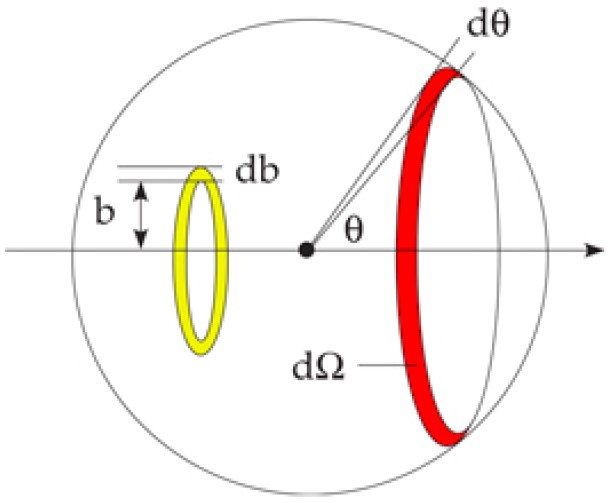
\includegraphics[width=150pt]{fig1_02}
\caption{Schematizzazione della sezione d'urto differenziale in base al parametro d'impatto e all'angolo solido.}
\label{fig:1.2}
\end{figure}
L'area delle particelle incidenti è data dalla formula $d\sigma=2\pi b |db|$. 
Le particelle definite in quest'area saranno diffuse all'angolo $d\Omega =2\pi \sin\theta d\theta$. 
Facendo il rapporto tra le due aree si ottiene la sezione d'urto differenziale dal punto di vista cinematico
\[\frac{d\sigma}{d\Omega}=\frac{b(\theta)}{\sin\theta}\frac{db}{d\theta}\]

Si può a questo punto unire le formule ricavando b rispetto a $\theta$ 
\[\frac{db}{d\theta}=\frac{d}{d\theta}\biggl|\frac{k}{\tan\frac{\theta}{2}}\biggl|=\frac{K}{\tan^2 \frac{\theta}{2}}\frac{1}{2}\frac{1}{\cos^2\frac{\theta}{2}}\]
\[\frac{d\sigma}{d\Omega}=\frac{1}{2}\frac{K^2}{\tan^3 \frac{\theta}{2}}\frac{1}{\cos^2\frac{\theta}{2}\sin^2\frac{\theta}{2}}=\frac{K^2}{4\sin^4\frac{\theta}{2}}\]
\[=\frac{1}{16}\left(\frac{zZe^2}{4\pi\varepsilon_0 T}\right)\frac{1}{\sin^4\frac{\theta}{2}}\]
Introduciamo quindi un po' di costanti che aiutano a semplificare questa formula e spesso usate in fisica subatomica
\[\alpha=\frac{b^2}{4\pi\varepsilon_0\hbar c}=\frac{1}{137}\hspace{1cm}\hbar c=197 MeV\cdot fm\]
dove $\alpha$ si definisce come costante di struttura fine. 
La formula con queste costanti diventa
\[\frac{d\sigma}{d\Omega}=\frac{z^2Z^2}{16}\alpha^2\left(\frac{\hbar c}{T(MeV)}\right)^2 \frac{1}{\sin^4\frac{\theta}{2}}\]
La cosa straordinaria di questa sezione d'urto sta nel fatto che, per delle coincidenze sotto un certo punto di vista fortuite, è uguale a quella calcolata con la meccanica quantistica. Questo succede perché nell'interazione di particelle alfa con il nucleo gli spin sono ininfluenti. 

Commenti alla sezione d'urto:
\begin{itemize}
\item La sezione d'urto diminuisce all'aumentare dell'energia cinetica (inversamente proporzionale a $T^2$.
\item Decresce rapidamente all'aumentare di $\theta$.
\item \'E proporzionale al quadrato delle cariche.
\end{itemize}


\subsection{Sezione d'Urto Quantistica (Regola d'Oro di Fermi)}
In meccanica quantistica quello che si introduce è che la probabilità d'interazione viene espressa dalla regola d'oro di Fermi
\[P=\frac{2\pi}{\hbar}|H_{f,i}|^2\rho(E_f)\]
I contributi che compongono questa probabilità d'interazione sono:
\begin{itemize}
\item $H_{f,i}$ è l'elemento dell'Hamiltoniana della perturbazione, ovvero la probabilità che la sezione d'onda iniziale passi alla sezione d'onda finale.
\[H_{f,i}=<f|H|i>=\int \psi*_f(r)H(\bar r)\psi_i d^3r\]
(La probabilità di passaggio di uno stato iniziale ad uno stato finale si valuta effettuando questo integrale tra lo stato iniziale e quello finale della Hamiltoniana di perturbazione).
Le funzioni d'onda sono quelle che descrivono le nostre particelle $\alpha$
\[H(r)=V(r)=\frac{zZe^2}{4\pi \varepsilon_0r}\]
Quali sono quindi gli stati (funzioni d'onda) che descrivono gli alfa?
Ad una certa distanza iniziale saranno onde piane
\[\psi_i \sim e^{ikr} \hspace{1cm}\bar p=\hbar\bar k\hspace{0.5cm}\bar k=\frac{\bar p}{\hbar}\]
Dopo l'interazione, ovvero quando le particelle non subiranno più il potenziale coulombiano, si avrà che la funzione sarà nuovamente un'onda piana ma con vettore d'onda variato (legato ovviamente alla quantità di moto)
\[\psi_i \sim e^{ik'r}\hspace{1cm} \bar p'=\hbar\bar k'\hspace{0.5cm}\bar k'=\frac{\bar p'}{\hbar}\]
Tornando alla regola d'oro di fermi, ciò mi dice che la probabilità d'interazione dipende dalla probabilità che il mio potenziale faccia passare le mie particelle da una certa quantità di moto ad un'altra.

\item L'altro contributo si ha dalla densità degli stati finali $\rho(E_f)$, ovvero il numero di stati finali acccessibili al sistema, maggiore è il tipo di capienza nello spazio delle fasi maggiore è la probabilità. Per ora trascureremo questo contributo per trattarlo più avanti.
\end{itemize}

Studiamo quindi la variabilità della probabilità in base alle funzioni d'onda. 
Si ha
\[H_{f,i}\simeq \int e^{-ik'r} V(r)e^{+ikr}=\int V(r)e^{-i(k'-k)r}\]
\[\bar p=\hbar \bar k \hspace{0.5cm} \bar p=\hbar k' \hspace{0.2cm}\to\hspace{0.2cm}\bar p' -\bar p =\Delta p=\bar q=\hbar (k'-k)\]
\[H_{f,i}=\int V(r) e^{-i\frac{\bar q}{\hbar}r}d^3r=\frac{zZe^2}{4\pi\varepsilon_0}\int \frac{1}{r}e^{-i\frac{\bar q}{\hbar}r}\]
Come si può vedere questa formula corrisponde ad una trasformata di Fourier, ciò che si ottiene alla fine è
\[H_{f,i}=\frac{zZe^2}{4\pi\varepsilon_0}\frac{4\pi\hbar^2}{q^2}\]
l'ultima frazione è la parte che si utilizza per calcolare la sezione d'urto differenziale
\[\frac{d\sigma}{d\Omega}\propto P\simeq |H_{f,i}|^2\sim\frac{1}{q^4}\]
Si può vedere poi che questa funzione, ricavata quantisticamente esprime la stessa dipendenza ricavata tramite metodo classico.
\[\bar{\Delta p}=\bar p'-\bar p=q=2p \sin\frac{\theta}{2}, \hspace{0.5cm}T=\frac{1}{2}mv^2\]
\[q^2=4m^2v^2\sin^2 \frac{\theta}{2}=8mT\sin^2\frac{\theta}{2}\]

Nella trattazione classica abbiamo supposto che le particelle non avessero interazioni di spin, abbiamo trascurato inoltre che i nuclei avessero rinculo. 
Queste sono due assunzioni buone ma che per risultati più precisi vanno considerate.
Si consideri ora il raggio nucleare stimato de Rutherford per la sua trattazione tramite scattering $\alpha$. 
Si cerchi la distanza di massimo avvicinamento della particella a nucleo, questa si avrà per un'energia pari a 
\[V=k\alpha \hspace{0.5cm}K=\frac{1}{4\pi\varepsilon_0}\frac{zZe^2}{R_0}\]
\[R_0=\frac{1}{4\pi\varepsilon_0}\frac{zZe^2}{k\alpha}\frac{\hbar c}{\hbar c}\simeq\frac{1}{137}\frac{2\cdot 79}{4\cdot 9 MeV}\hbar c =46 fm\]
Questa è una sovrastima del raggio nucleare in quanto si sa attualmente che il raggio corrisponde ad 8 fermi. 
Questo errore è dovuto al fatto che non vi è interazione nucleare nello scattering di Rutherford ma semplicemente elettrostatica, il che spiega anche la perfetta corrispondenza dei suoi dati con la trattazione teorica. 
Supponiamo quindi di riuscire ad aumentare l'energia delle particelle $\alpha$ (quello che accade negli acceleratori). 
Si supponga poi di utilizzare come target del piombo e di porre un rivelatore a 60°. 
Si può osservare che l'andamento del numero di particelle scatterate per energie inferiori a 27,5 MeV rispecchia esattamente l'andamento di Rutherford ma poi ha un cambio drastico. 
Questo accade perché oltre un certo raggio subentra l'interazione per forza forte
\[R=\frac{Q_1Q_2}{4\pi\varepsilon_0KE}=8.59 fm\]
La sovrastima di Rutherford era dovuta al fatto che le particelle da lui usate avevano effettivamente interazione puramente coulombiana.